\documentclass[12pt]{article}

\usepackage{sbc-template}
\usepackage{graphicx,url}
\usepackage[utf8]{inputenc}
\usepackage[brazil]{babel}
\usepackage{verbatim}
\usepackage[final]{pdfpages}
%\usepackage[latin1]{inputenc}

% 19/06: http://sbrt.org.br/sbrt2020/cfp.html#cfp
% 01/07: http://voyager.ce.fit.ac.jp/conf/3pgcic/2020/
% 10/07: http://sbseg.sbc.org.br/2020/pt/chamadas/principal.html
% 14/07: http://conferences.cis.umac.mo/pdcat20/
     
\usepackage{xspace}
\newcommand{\FC} {Freechains\xspace}

\newcommand{\Xon} {$1{\rightarrow}N$\xspace}
\newcommand{\Xno} {$1{\leftarrow}N$\xspace}
\newcommand{\Xnn} {$N{\leftrightarrow}N$\xspace}
\newcommand{\Xoo} {$1{\leftrightarrow}1$\xspace}
\newcommand{\Xo}  {$1{\hookleftarrow}$\xspace}

\sloppy

\begin{comment}
http://sbseg.sbc.org.br/2020/pt/chamadas/ferramentas.html
- Descrição da demonstração planejada para o Salão de Ferramentas, informando equipamentos necessários para tal;

    - public key cryptography to deal with identities, confidentiality and
\end{comment}


\title{\FC: Disseminação de Conteúdo Peer-to-Peer}

\author {
    Francisco Sant'Anna,
    Fabio Bosisio,
    Lucas Pires
}
\address {
    UERJ - Departamento de Ciência da Computação
    \email{francisco@ime.uerj.br, fbosisio@gmail.com, lucasampires@gmail.com}
}

\begin{document} 

\maketitle

\begin{abstract}
O \FC é um sistema peer-to-peer para disseminação de conteúdo: um
usuário posta uma mensagem em um tópico e seus assinantes eventualmente recebem
a mensagem.
As postagens são estruturadas em um grafo direcionado acíclico criptográfico
que é imune a modificações (\emph{Merkle DAG}).
O grafo é disseminado par a par na rede por \emph{gossip} de maneira não
estruturada.
O \FC suporta múltiplos arranjos de disseminação pública e privada entre grupos
e indivíduos, sendo possível modelar desde conversas privadas por e-mail, até
debates entre desconhecidos em fóruns públicos.
Cada tópico público conta com um sistema descentralizado de reputação para
combater abusos, tais como SPAM e notícias falsas.
%Autores precisam de reputação prévia para postar novo conteúdo, que ainda assim
%pode ser removido se a proporção entre \emph{likes \& dislikes} for muito baixa.
O \FC executa como um \emph{daemon} nos pares da rede e pode ser acessado pela
linha de comando, API em Kotlin ou sockets.
\end{abstract}
     
%\begin{resumo}
%\end{resumo}

\section{Introdução}

Apesar do crescimento contínuo da internet ao longo dos anos, o conteúdo
disseminado está cada vez mais sob o controle de poucas
empresas~\cite{internet.fixing}.
Consideramos como disseminação de conteúdo qualquer tipo interação na internet,
tais como trocas de e-mails, consumo de notícias, diálogos em redes sociais,
ou até mesmo backup de documentos.
%
As empresas de internet tipicamente são somente intermediárias entre seus
usuários, mas não criam conteúdo original.
Por um lado, elas são essenciais, oferecendo interfaces amigáveis,
armazenamento grátis e conectividade permanente.
Por outro lado, essas empresas concentram mais poder do que o necessário para
operarem, uma vez que controlam nossos dados, coletam informações privadas,
``algoritimizam'' o consumo, e ainda dificultam a portabilidade entre serviços
através de formatos e protocolos proprietários.

Sistemas de disseminação \emph{peer-to-peer}~\cite{p2p.survey} oferecem uma
alternativa aos serviços centralizados, eliminando intermediários e movendo
para os usuários finais toda a responsabilidade pela transferência,
armazenamento, disponibilidade e validação do conteúdo disseminado.
No entanto, há diversos novos desafios, tais como distribuir adequadamente a
infraestrutura de conectividade e armazenamento, lidar com pares (\emph{peers})
maliciosos na rede, e investir na usabilidade do sistema sem um modelo de
negócio.

Neste trabalho, apresentamos o \emph{\FC} como uma ferramenta para a
disseminação de conteúdo peer-to-peer sem intermediação ou controle de acesso
centralizado, e sem a necessidade de confiança entre seus usuários.
No \FC, um usuário posta uma mensagem em um tópico, também chamado de
cadeia, e todos os outros assinantes alcançáveis na rede peer-to-peer
eventualmente recebem a mensagem.
O \FC apresenta duas contribuições principais: (1) um protocolo mínimo para
múltiplos arranjos de disseminação de conteúdo e (2) um sistema de reputação
autônomo e descentralizado.
%
Sobre a primeira contribuição, a Figura~\ref{fig.table} descreve os diversos
arranjos de disseminação entre seus usuários:
    arranjos públicos \Xon e \Xno,
    arranjos privados \Xoo, \Xnn e \Xo, e
    arranjos públicos \Xnn.
%
\begin{comment}
\begin{itemize}
\item Arranjos públicos \Xon e \Xno:
    Uma identidade pública (ex., pessoa ou organização) dissemina conteúdo
    autenticado para um público alvo (\Xon) com feedback opcional (\Xno).
    Exemplos são sites de notícias, serviços de streaming e perfis públicos em
    redes sociais.
\item Arranjos privados \Xoo, \Xnn e \Xo:
    Grupos de confiança (ex., amigos ou familiares) trocam mensagens privadas
    entre si.
    A comunicação pode ser em pares (\Xoo), grupos (\Xnn) ou até mesmo
    individuais (\Xo).
    Exemplos são e-mails, grupos de família e backup de documentos.
\item Arranjos públicos \Xnn:
    Grupos heterogêneos se comunicam publicamente. Exemplos são fóruns de
    perguntas e respostas, chats, e compra \& venda online.
\end{itemize}
\end{comment}
%
%A API do protocolo é composta basicamente de comandos para assinar cadeias de
%interesse (\texttt{join}), postar novas mensagens (\texttt{post}), iterar sobre
%mensagens existentes (\texttt{traverse}), e ler uma mensagem específica
%(\texttt{get}).
%
Sobre a segunda contribuição, o sistema de reputação do \FC rege a qualidade
das postagens e autores dentro de cadeias públicas e tem os seguintes
objetivos:
%
\begin{itemize}
\item Combater o excesso de conteúdo restringindo o número de postagens por autor.
\item Destacar o conteúdo de qualidade com um mecanismo de \emph{likes \& dislikes}.
\item Combater SPAM, notícias falsas e conteúdo ilícito exigindo reputação
      prévia de autores e removendo postagens com proporção muito baixa entre
      likes e dislikes.
\end{itemize}
%
O código fonte, documentação e vídeos introdutórios sobre o \FC estão
disponíveis em \url{https://github.com/Freechains/README}.
%A ferramenta pode ser demonstrada em um vídeo pré-gravado com a simulação de
%uma rede peer-to-peer com pares conectados via SSH.

\begin{figure}[ht]
\centering
%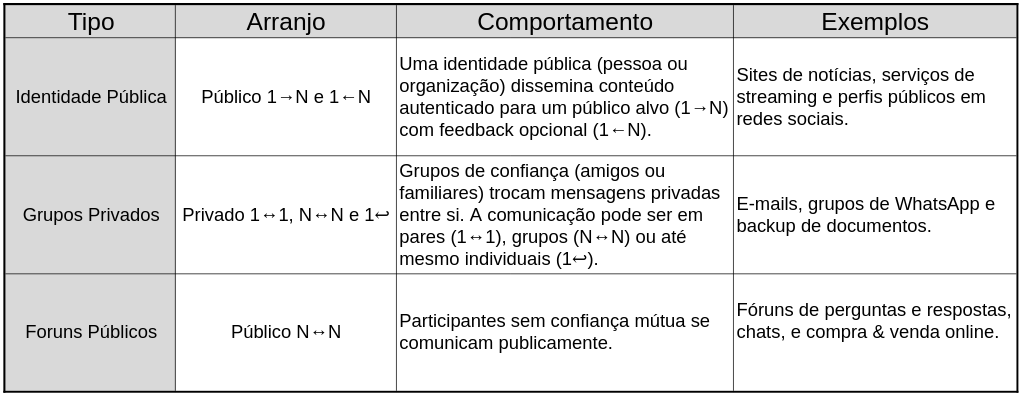
\includegraphics[width=\textwidth]{arranjos}
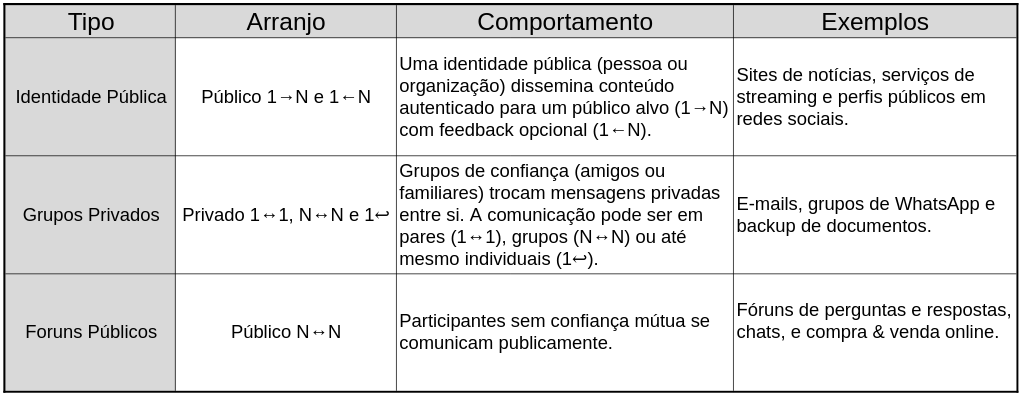
\includegraphics[width=\textwidth]{arranjos.png}
%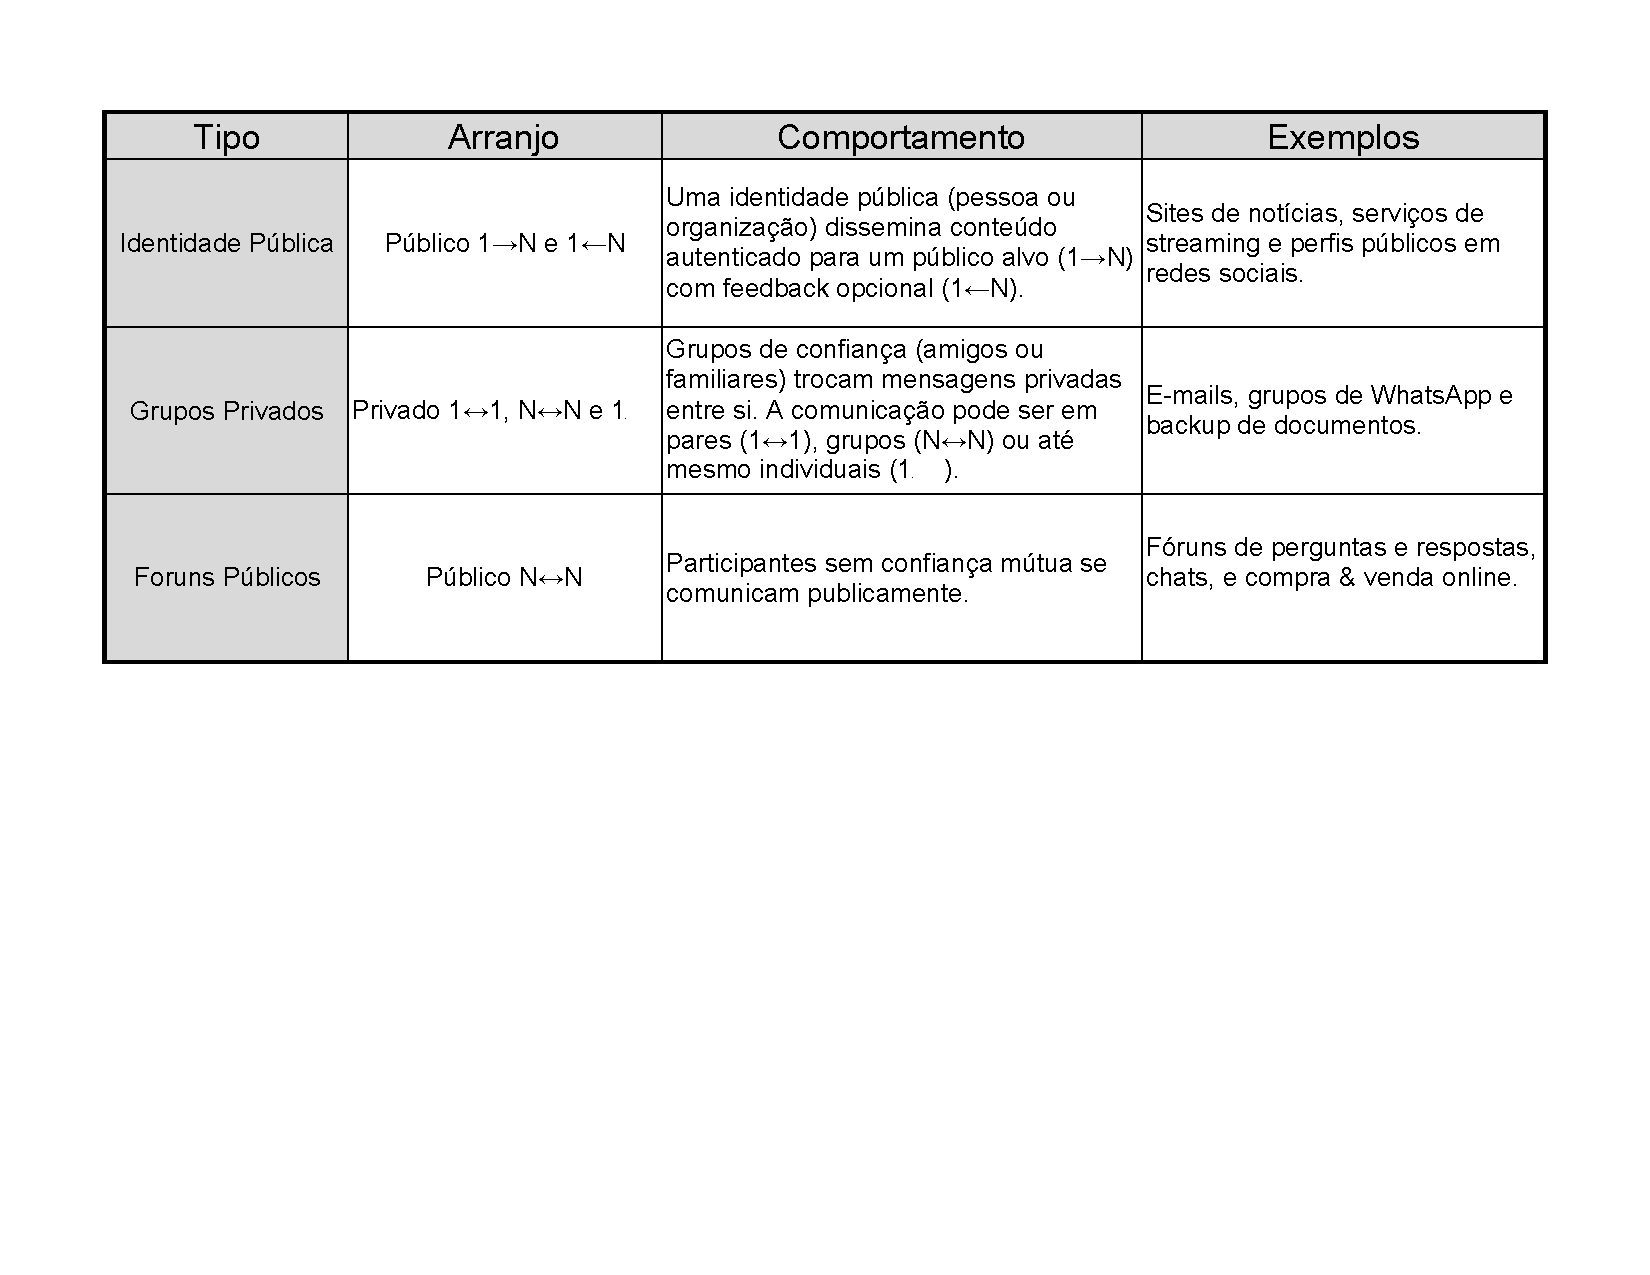
\includegraphics[clip, trim=1.75cm 10.25cm 1.5cm 1.75cm, width=1.00\textwidth]{arranjos.pdf}
%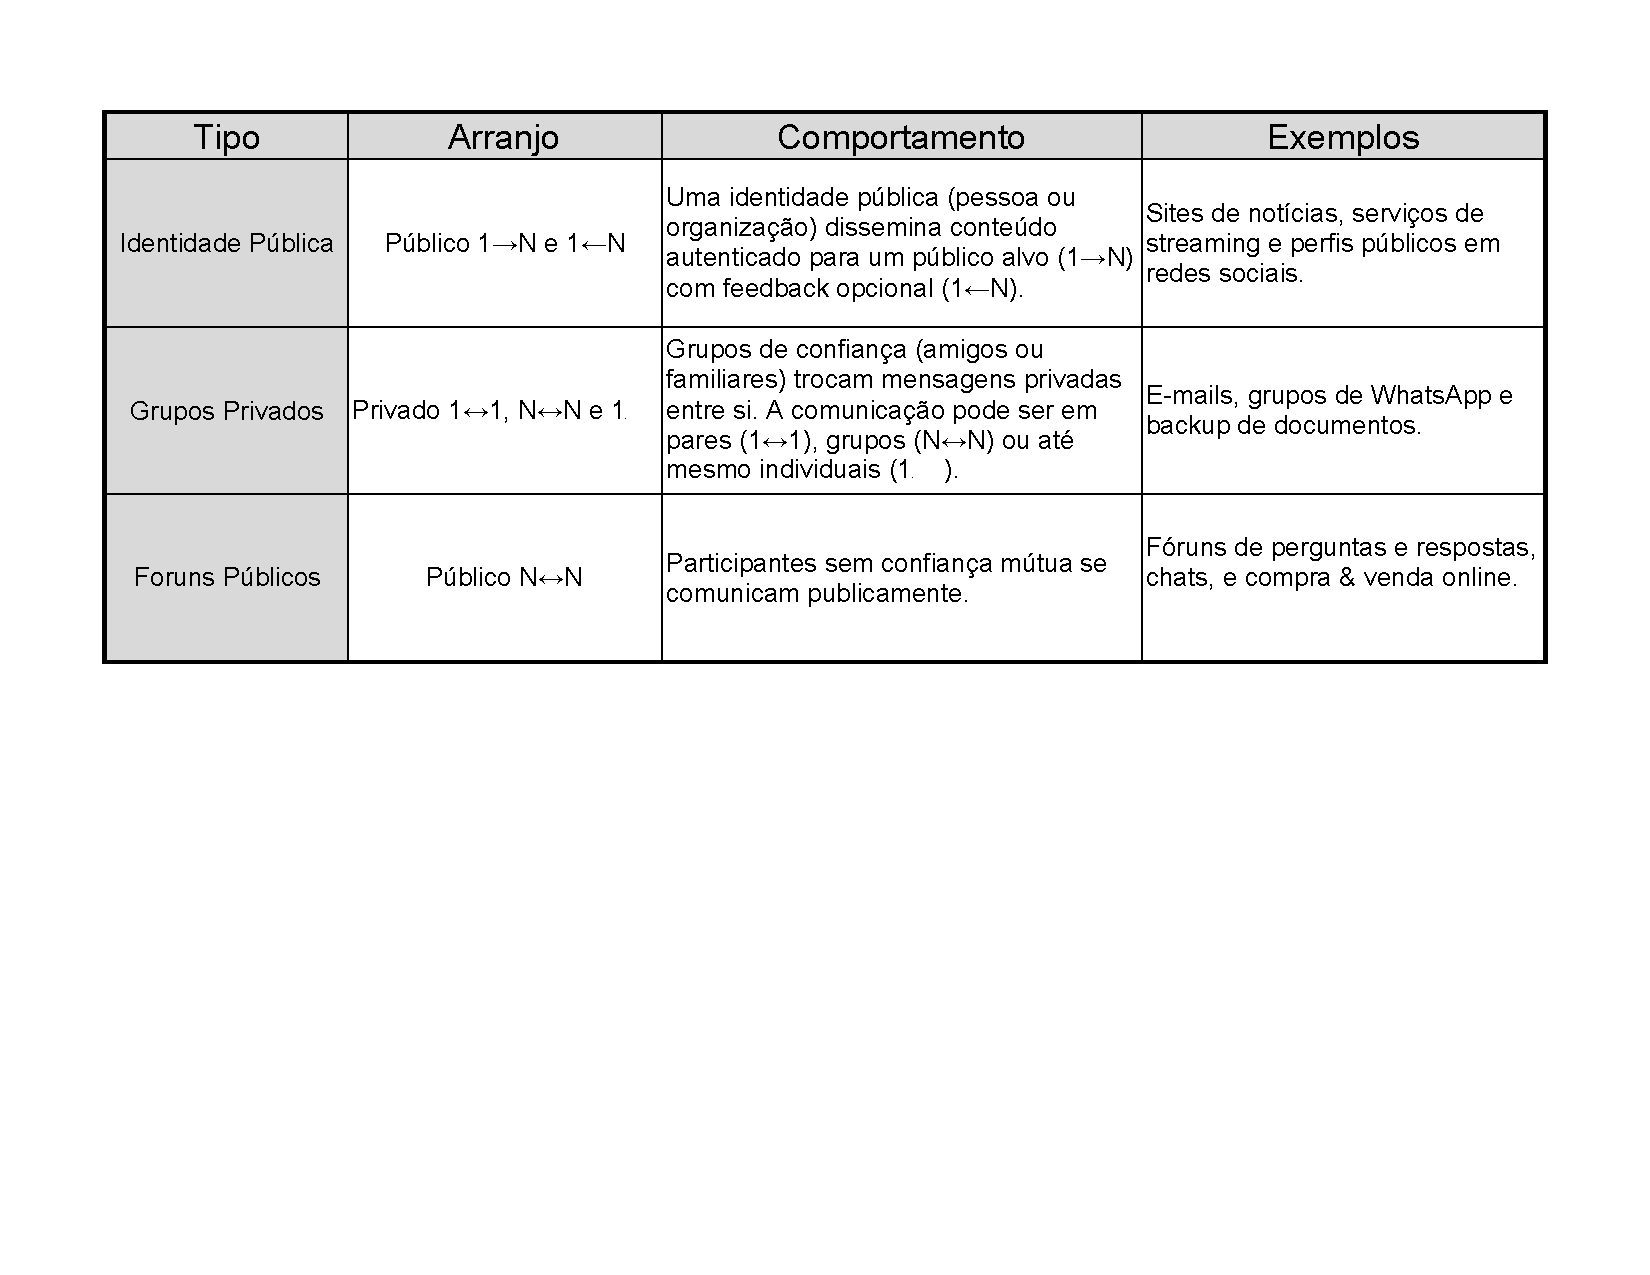
\includepdf[width=\textwidth]{arranjos.pdf}
%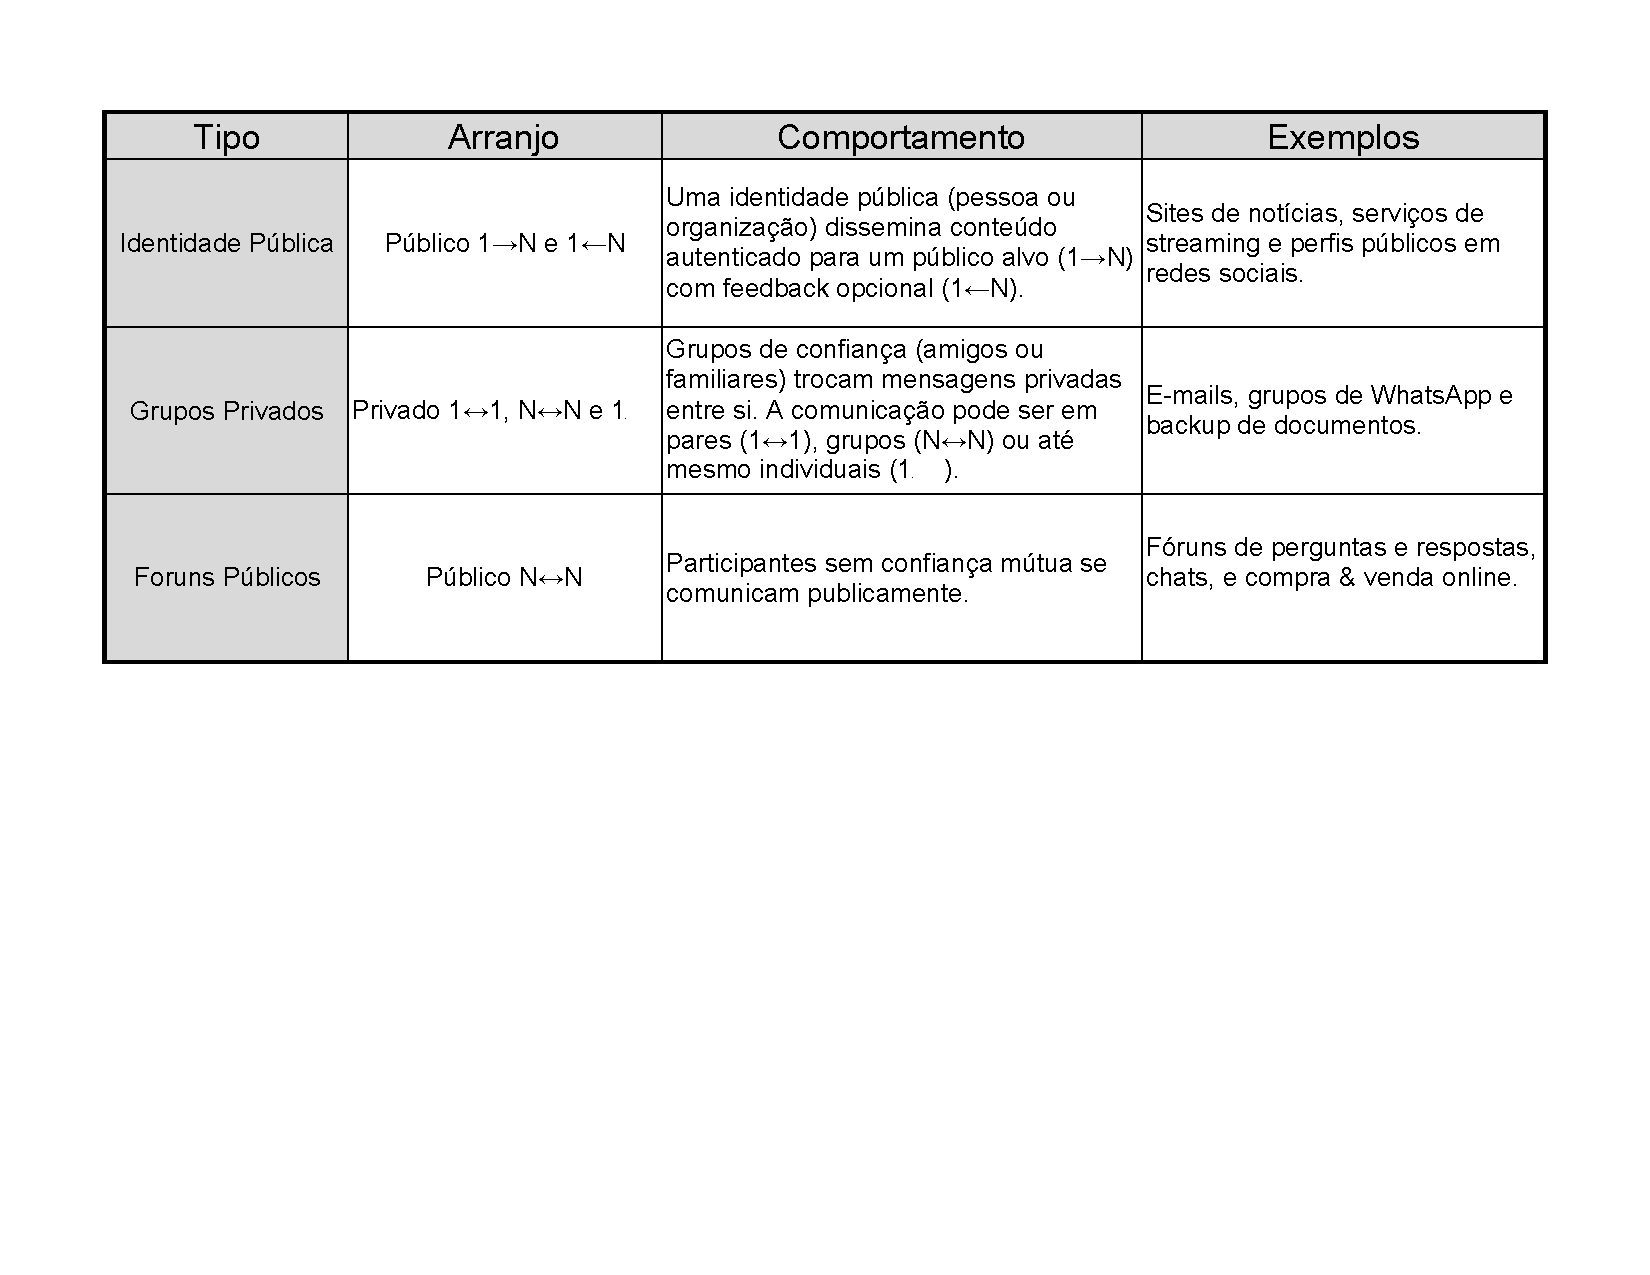
\includepdf[pages=-,pagecommand={},width=\textwidth]{arranjos.pdf}
\caption{Os 3 tipos de cadeias e arranjos do \FC}
\label{fig.table}
\end{figure}

A Seção~\ref{sec.related} compara o \FC com sistemas \emph{pubsub}, protocolos
federados e outras aplicações peer-to-peer.
A Seção~\ref{sec.freechains} apresenta o funcionamento básico do \FC além de
uma discussão sobre os arranjos de disseminação e o sistema de reputação.
A Seção~\ref{sec.conclusion} conclui o trabalho.

\section{Comparação com Outros Sistemas}
\label{sec.related}

%Diversos sistemas oferecem disseminação de conteúdo de forma distribuída.
%Aqui nós consideramos \emph{middlewares publish-subscribe},
%\emph{protocolos federados} e \emph{sistemas peer-to-peer completos}.

%\subsection{Middlewares Publish-Subscribe}

Os middlewares publish-subscribe desacoplam produtores (\emph{publishers}) de
consumidores (\emph{subscribers}) através de um intermediário (\emph{broker}).
Exemplos de sistemas \emph{pubsub} incluem o \emph{XMPP}, \emph{AMQP},
\emph{WebSub} e \emph{ActivityPub}.
Uma limitação chave em pubsubs é que, embora produtores e consumidores
se comuniquem sem conhecimento mútuo, os brokers ainda possuem um papel
centralizador na rede.
Eles são necessários para autenticar e validar as postagens, por exemplo, além
de hospedarem as filas de mensagens que conectam produtores e consumidores.
%As filas são hospedadas em endereços previamente conhecidos (ex.,
%\url{amqp://user@domain/path}), o que impede uma arquitetura inteiramente
%distribuída.

\begin{comment}
Aumentar o número de servidores, como em pubsubs federados~\cite{TODO} não
afeta o modelo fundamentalmente, uma vez que cada fila se mantém independente e
serve as ações dos seus clientes isoladamente.
A peça ausente na arquitetura pubsub para torná-la totalmente descentralizada é
uma política para mesclar filas independentes, de modo que as localidades
específicas dos brokers possa variar dinamicamente sem afetar o funcionamento
do sistema.
Os problemas de sincronizar os brokers de alguma maneira são similares aos que
o \FC se propõe a resolver: como ordenar e relacionar mensagens em
múltiplos servidores, como lidar com excesso de conteúdo e SPAM, como lidar com
notícias falsas, conteúdo legal e etc.
\end{comment}

%\subsection{Protocolos e Aplicações Federadas}

Em protocolos federados, múltiplos servidores se sincronizam para permitir a
comunicação externa entre seus usuários, mas a identidade de um usuário ainda é
atrelada a um servidor específico.
Todo conteúdo poder ser gerenciado localmente nas instâncias da federação e a
sincronização externa é um passo em separado, mas que não é necessário para o
funcionamento local.
%
O serviço de e-mail (SMTP) é provavelmente o protocolo federado mais popular e
permite que usuários de domínios diferentes troquem mensagens de maneira
transparente.
Mais recentemente, os sistemas \emph{Diaspora}, \emph{Matrix} e \emph{Mastodon}
cobriram aos cenários de redes sociais, chats e \emph{microblogging} com
arquiteturas federadas.
%No entanto, a identidade de um usuário não é portável, ou seja, está atrelada a
%um servidor específico e não pode ser usada transparentemente em outros.
%, que inclusive podem ter homônimos ativos.
No entanto, sem o controle de sua própria identidade, um usuário fica refém do
seu servidor na federação.
Por exemplo, o servidor pode ser desligado pelos seus administradores ou banido
pelo resto da federação, ou ainda o próprio usuário pode ficar insatisfeito com
o serviço prestado.
Em qualquer um desses casos, o usuário terá que exportar todo o seu conteúdo e
histórico para outro servidor e anunciar a sua nova identidade aos seus
seguidores.

\begin{comment}
Em sistemas peer-to-peer como propomos com o \FC, a identidade é
controlada pelo próprio usuário com autenticação de chave pública, que pode ser
usada igualmente em qualquer par da rede.
A moderação de conteúdo é uma outra preocupação em sistemas federados.
Como exemplo, mensagens que atravessam os limites da sua federação estão
sujeitos a políticas diferentes.
Tipicamente, as regras de moderação podem ser aplicadas localmente pelo usuário
(ex., filtros de e-mail) ou ainda por servidores, o que afeta todos os seus
usuários.
O primeiro caso é mais flexível, porém é sujeito a ataques de disparo de
mensagens em massa, por exemplo.
O segundo caso pode bloquear o acesso a mensagens legítimas, pois ações globais
são potencialmente sempre mais restritivas.
No \FC, a moderação ocorre em outra dimensão.
Em vez de indivíduos ou servidores adotarem políticas verticais em todas as
suas mensagens, o \FC aplica uma política horizontal por tópico que
afeta a sua disseminação na rede peer-to-peer inteira.
Essa política parte do princípio que uma mensagem que é indesejada em uma
comunidade não necessariamente será indesejada em outras comunidades.
Como um contraponto, protocolos federados são mais apropriados para aplicações
de tempo real com um grande número de mensagens curtas, tais como chats e
streaming.
A quantidade de saltos e sobrecarga de cabeçalho pode ser bem menor em
arquiteturas cliente-servidor em comparação com sistemas peer-to-peer, que
tipicamente dependem de assinaturas digitais, \emph{hash linking} e
verificações extras.
\end{comment}

%\subsection{Sistemas Peer-to-Peer}

Em sistemas peer-to-peer, todos os pares da rede desempenham as mesmas funções
e atuam ora como clientes, ora como servidores.
O \emph{Bitcoin}~\cite{p2p.bitcoin} é provavelmente a rede peer-to-peer de
maior sucesso, mas serve ao propósito único de uma criptomoeda descentralizada,
não sendo adequado para comunicações genéricas entre pares.
O \emph{Scuttlebutt}~\cite{p2p.scuttlebutt} e
\emph{Aether}\footnote{\url{https://getaether.net/}~(acessado em Jul/2020)} atendem aos cenários de
comunicação entre amigos e grupos, focando respectivamente, na comunicação
pública \Xon e \Xnn.
\begin{comment}
Já o IPFS~\cite{p2p.ipfs} e Dat~\cite{p2p.dat} oferecem hospedagem de arquivos
e aplicações.
O IPFS é baseado no conceito de dados imutáveis com endereçamento por conteúdo,
enquanto que o Dat em dados mutáveis com endereçamento por chave pública.
O IPFS é mais adequado para compartilhar arquivos grandes e estáveis, tais como
filmes e versões de software, enquanto que o Dat, para conteúdo dinâmico como
aplicações web.
Ambos usam \emph{DHTs} como base de suas arquiteturas, sendo portanto
otimizadas para servir conteúdos grandes e populares, mas não tanto para buscas
e descobrimento de conteúdo novo~\cite{p2p.survey}.
%Ambos também requerem que os usuários saibam de antemão o endereço do conteúdo,
%seja o link exato de um filme, seja uma identidade em particular da rede.
Por essa razão, DHTs não são a melhor arquitetura para modelar atualizações
contínuas de conteúdo com múltiplos autores, tais como em fóruns públicos.
%Os sistemas a seguir não usam DHTs em sua arquitetura.
O Bitcoin tem uma propriedade muito forte de garantir que as mensagens da rede
são ordenadas e que essa ordem é exatamente a mesma em todos os pares, ou seja,
que há um consenso global sobre o estado da rede.
O Bitcoin usa um algoritmo de consenso baseado em prova de trabalho que é imune
a ataques \emph{sybil} em que identidades são forjadas.
No entanto, prova de trabalho é computacionalmente cara e, na prática, mantém a
rede sob controle de poucos pares, afetando o objetivo principal de
descentralização.
O \FC usa um sistema de reputação próprio para evitar SPAM e ataques
sybil.
O sistema é apresentado na Seção XX e pode ser entendido como uma prova de
trabalho para humanos: um autor precisa “trabalhar” para postar conteúdo de
qualidade por sua vez é avaliado por outros humanos.
Dentre os trabalhos discutidos, o Scuttlebutt e Aether são os mais similares ao
\FC, e focam, respectivamente, na comunicação pública \Xon e \Xnn.
\end{comment}
O Scuttlebutt é baseado em identidades de usuários que se seguem par a par e
formam um grafo que se reflete tanto nas conexões de rede quanto no
armazenamento redundante dos seus dados.
%Como exemplo, se a identidade \emph{A} segue a identidade \emph{B}, então o
%computador de \emph{A} se conecta diretamente ao computador de \emph{B} e
%também armazena todas as postagens de \emph{B} localmente.
%As relações são assimétricas, permitindo que \emph{B} não siga \emph{A}
%necessariamente no exemplo dado.
%A topologia de rede do \FC também se baseia em conexões par a par, mas
%não necessariamente entre seguidores.
Já o Aether se organiza em comunidades em torno de tópicos, com postagens
replicadas na rede, mas que são efêmeras considerando uma janela de tempo.
O Aether usa prova de trabalho nas postagens para evitar SPAM e elege
moderadores para prevenir comportamento abusivo.%
\footnote{{\tiny{\url{https://blog.getaether.net/post/187829323237/aether-p2p-dev14-released-with-moderation}}}~(acessado em Jul/2020)}
%
O \FC também se baseia em tópicos, mas como um tópico pode ser de propriedade
de uma identidade, então é possível modelar o comportamento dos dois sistemas.
Além disso, introduz um sistema de reputação distribuído para lidar com abuso
conforme discutido na Seção~\ref{sec.freechains.reps}.

\section{Visão Geral do \FC}
\label{sec.freechains}

\subsection{Funcionamento Básico}

O \FC é um sistema publish-subscribe baseado em tópicos: um usuário
posta uma mensagem em um tópico e seus assinantes eventualmente recebem a
mensagem.
A Figura~\ref{fig.all} ilustra os quatro conceitos básicos do \FC:
\emph{cadeias}, \emph{blocos}, \emph{autores} e \emph{pares}.

\begin{figure}[ht]
\centering
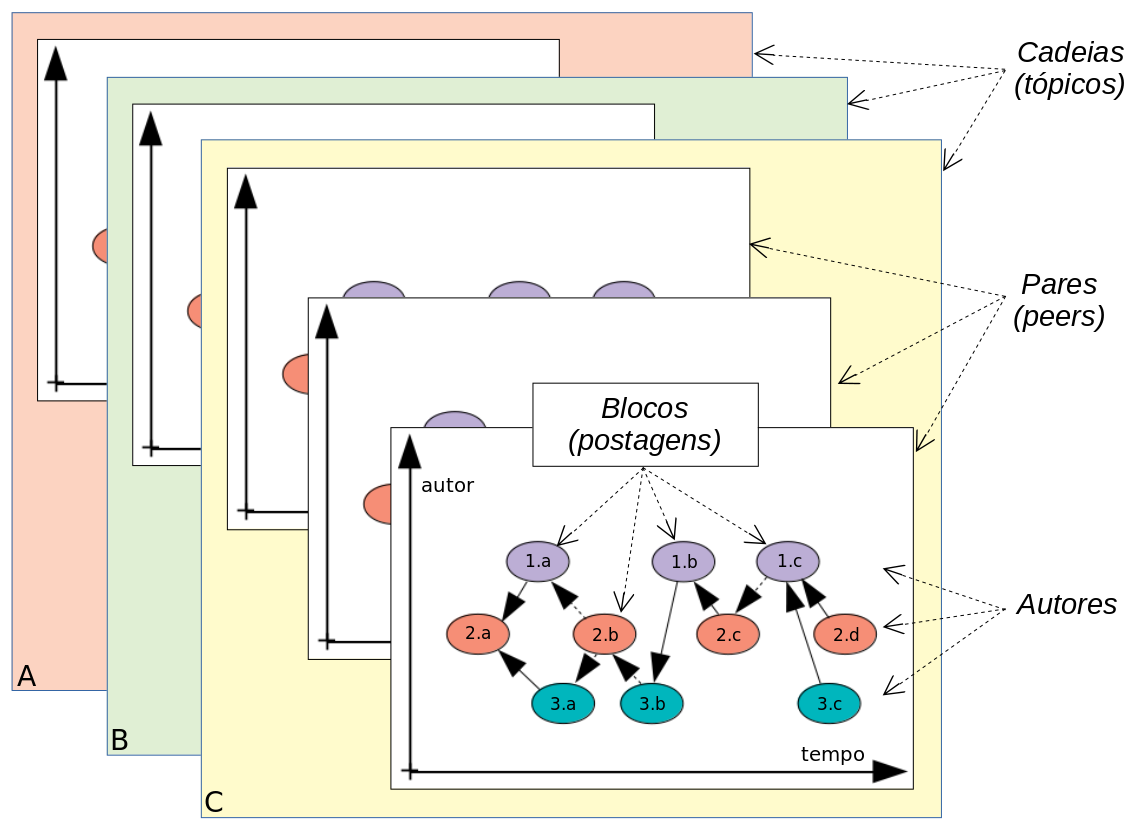
\includegraphics[width=.60\textwidth]{all3.png}
\caption{\scriptsize{Conceitos básicos do \FC: cadeias, blocos, autores e pares.}}
\label{fig.all}
\end{figure}

As \emph{cadeias}, destacadas em quadrados coloridos (vermelho/A, verde/B e
amarelo/C), são independentes umas das outras e podem representar, por exemplo,
os \emph{tweets} de uma celebridade (arranjo \Xon público), um grupo de
\emph{Whatsapp} de amigos (arranjo \Xnn privado) ou um \emph{subreddit} de um
tema qualquer (arranjo \Xnn público).

Cada cadeia possui um conjunto de \emph{blocos} com suas postagens, que estão
destacadas como elipses coloridas (roxo/1.x, vermelho/2.x e verde/3.x), em que
cada cor representa um \emph{autor}.
Os blocos da cadeia formam um grafo de causalidade indicando a relação temporal
entre elas.
Por exemplo, a primeira mensagem do autor vermelho (\texttt{2.a}) ocorreu antes
das primeiras mensagens dos autores roxo e verde (\texttt{1.a} e \texttt{3.a}).
O grafo é um DAG e expressa a ordem parcial entre todos os blocos na cadeia.
Toda cadeia tem um bloco \emph{gênesis} preexistente (não exibido na imagem)
que, por construção, é alcançável por todos os blocos da cadeia.

O grafo da cadeia é inteiramente replicado em todos os pares.
%com assinantes, ou seja, todos
%mantém todas as mensagens da cadeia, independentemente da autoria das
%postagens.
Na figura, a cadeia amarela/C é replicada em três pares.
A disseminação do grafo pela rede é feita por \emph{gossip}, ou seja, os pares
se conectam dois a dois para sincronizar os seus grafos.
Dessa maneira, o recebimento de mensagens no pares é eventual, pois depende de
um roteamento par a par da origem ao destino.

O \FC executa como um servidor ou \emph{daemon} e escuta requisições de
usuários locais, por exemplo para postar ou ler mensagens, e também se comunica
com outros pares da rede peer-to-peer para sincronizar as suas cadeias de
interesse.
O daemon pode ser acessado de três formas equivalentes:
%
\begin{itemize}
\item Pela linha de comando, que usamos no resto do artigo.
\item Por uma API em Kotlin, linguagem da implementação de referência.
\item Por um protocolo textual, que permite usar outras linguagens via sockets.
\end{itemize}
%
\begin{comment}
% 
Os principais comandos do \FC são enumerados a seguir:
%
\begin{itemize}
\item {\footnotesize\texttt{freechains-host start}}:     inicia daemon no diretório passado
\item {\footnotesize\texttt{freechains crypto}}:         cria identidade criptográfica
\item {\footnotesize\texttt{freechains chains join}}:    inscreve-se na cadeia
\item {\footnotesize\texttt{freechains chain post}}:     posta na cadeia
\item {\footnotesize\texttt{freechains chain get}}:      lê postagem da cadeia
\item {\footnotesize\texttt{freechains chain traverse}}: itera sobre a cadeia
\item {\footnotesize\texttt{freechains peer send/recv}}: sincroniza com par da rede
\end{itemize}
%
Exceto pelo comando para iniciar o daemon, os outros comandos principais são
efetuados remotamente através do cliente \texttt{freechains}.
Isso permite compartilhar um par da rede entre múltiplos clientes, por exemplo,
um desktop e um celular.
\end{comment}
%
A sequência de comandos a seguir ilustra o funcionamento básico do \FC:

{\footnotesize
\begin{verbatim}
$ freechains start /var/fcs/ &      # inicia daemon em background
$ freechains crypto pubpvt "senha"  # cria identidade publica
EB172E... 96700A...                 # (retorna chaves publica e privada)
$ freechains chains join "#chat"    # se inscreve na cadeia #chat
$ freechains chain "#chat" post inline "Bom Dia!" --sign=96700A...
\end{verbatim}
}

Após iniciar o daemon, o usuário cria uma identidade para si.
A chave pública pode ser compartilhada e a chave privada deve ser guardada em
segredo.
Em seguida o usuário se inscreve na cadeia \texttt{\#chat} e posta uma mensagem
assinando-a com a sua chave privada.
Até aqui, tudo ocorre localmente na máquina com o daemon em execução.
A comunicação com outros pares deve ser feita explicitamente:

{\footnotesize
\begin{verbatim}
$ freechains peer 10.0.0.2 send "#chat"  # envia  #chat para 10.0.0.2
$ freechains peer 10.0.0.2 recv "#chat"  # recebe #chat  de  10.0.0.2
\end{verbatim}
}

Note que o \FC não monta a topologia da rede peer-to-peer automaticamente.
Não há pares pré-configurados, não há \emph{root servers}, não há nenhum tipo
de descobrimento automático de pares.
As conexões se dão somente através dos comandos \texttt{send} e \texttt{recv}
que devem especificar os pares explicitamente.
Nesse sentido, o protocolo dá o suporte básico para a comunicação par a par,
mas a montagem da topologia da rede propriamente dita deve ser feita por fora
do protocolo.

Para ler as postagens de uma cadeia, primeiro identificamos os blocos não
lidos:

{\footnotesize
\begin{verbatim}
$ freechains chain "#chat" genesis                # hash id do genesis
0_10EEB7...
$ freechains chain "#chat" traverse all 0_10EE... # do genesis em diante
1_A5EF... 2_1B5C... 2_2144...
$ freechains chain "#chat" get payload 1_A5EF...  # conteudo do bloco
Bom dia!
\end{verbatim}
}

O comando \texttt{traverse} retorna todos os blocos mais novos que o(s)
bloco(s) passados como parâmetro e serve para identificar as postagens que
ainda não foram lidas.
Esse controle deve ser feito pelo usuário local, ou seja, este deve manter uma
lista dos seus últimos blocos lidos e passá-los para o \texttt{traverse} que
irá retornar os blocos recebidos ainda mais novos.
Inicialmente, usamos a identificação do bloco gênesis como âncora, já que
nenhum bloco ainda foi lido pelo usuário.
Em seguida, é possível usar o comando \texttt{heads} para identificar os blocos
mais novos na cabeça do grafo (que foram os lidos agora) e usá-los como âncora
na próxima varredura.
%
Uma outra forma é checar o conteúdo em tempo real através do comando
\texttt{listen}:

{\footnotesize
\begin{verbatim}
$ freechains chain "#chat" listen   # escuta novos blocos em tempo real
1_A5EF...                           # 1o bloco recebido
2_1B5C...                           # 2o bloco recebido
2_2144...                           # 3o bloco recebido
\end{verbatim}
}

O comando é bloqueante e exibe uma nova linha sempre que um novo bloco chega
com a sua identificação.
Esse comando pode ser usado em conjunto com um \emph{pipe} para reagir a novas
mensagens em tempo real.

Os comandos \texttt{send} e \texttt{recv} devem ser executados para cada cadeia
e para cada par da rede de interesse.
Por exemplo, se o usuário segue 10 cadeias e se liga a 5 pares, os comandos
deverão ser executados 100 vezes a cada sincronização ($2\times10\times5$).
O \FC inclui uma ferramenta para automatizar o processo inteiro de
sincronização.
É possível registrar pares e cadeias e a ferramenta usa internamente os
comandos \texttt{listen}, \texttt{send} e \texttt{recv} para se sincronizar
assim que uma nova mensagem é postada ou recebida.

Um bloco é uma estrutura de dados que persiste uma única mensagem na cadeia.
Ele se encadeia às postagens anteriores e é encadeado pelas próximas postagens.
A Figura~\ref{fig.block} ilustra o encadeamento de blocos no grafo da cadeia e
mostra a representação interna de um bloco com quatro campos enumerados:

\begin{enumerate}
\item[msg:]  O conteúdo da mensagem propriamente dita.
\item[sign:] Uma assinatura opcional com a chave pública do autor e o código da
             assinatura.
\item[meta:] Os metadados da mensagem: tempo de criação, se está criptografada,
             hash da mensagem, se é um like/dislike, e os elos para blocos
             anteriores.
\item[hash:] O hash criptográfico dos metadados do bloco que o identificam
             univocamente. O hash é prefixado com a altura do bloco na cadeia.
             Por exemplo, o bloco
                {\scriptsize\texttt{5\_F700CC98A6BA6A562CF6272AFC1044CB0F049E2E71D1076DA3391E85EE2CE2B8}}
             possui altura \texttt{5} e hash \texttt{F700CC...}.
\end{enumerate}

\begin{figure}[ht]
\centering
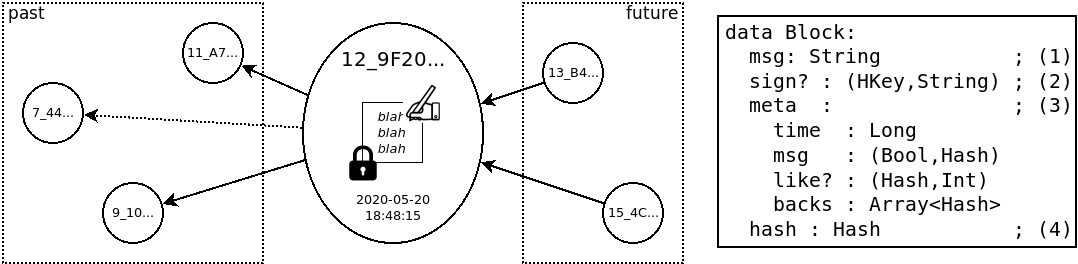
\includegraphics[width=.90\textwidth]{block1.png}
\caption{\scriptsize{Bloco (centro) se encadeia aos anteriores (esq.) e é encadeado
         pelos próximos (dir.).}}
\label{fig.block}
\end{figure}

O encadeamento dos blocos forma um grafo direcionado acíclico que é imune a
modificações (\emph{Merkle DAG}).
Ao se criar um novo bloco, calcula-se o hash dos seus metadados, que por sua
vez incluem os hashes da mensagem em si e dos blocos anteriores.
Esse novo hash identifica o bloco em todas as operações, inclusive nos elos dos
próximos blocos, e pode a qualquer momento ser recalculado para verificar se os
dados sofreram modificações.
Como os elos anteriores também são identificados da mesma forma, o grafo pode
ser verificado até o seu gênesis, cujo hash depende somente dos parâmetros da
cadeia, sendo igualmente verificável.

\subsection{Arranjos de Disseminação de Conteúdo}

O \FC oferece três tipos de cadeia, conforme apresentado na
Figura~\ref{fig.table}: identidade pública, grupos privados e fóruns públicos.
%
\begin{comment}
O \FC suporta três tipos de cadeias, cada uma com um propósito diferente:
%
\begin{itemize}
\item \textbf{Fóruns Públicos}:
    Arranjo \Xnn público.
    Comunicação pública entre participantes sem confiança mútua.
    Exemplos: fóruns de perguntas e respostas, chats, e compra \& venda online.
\item \textbf{Grupos Privados}:
    Arranjos privados \Xoo, \Xnn e \Xo.
    Comunicação privada entre pares, grupos ou individuais.
    Exemplos: e-mail, grupos de WhatsApp, backup.
\item \textbf{Identidade Pública}:
    Arranjos públicos \Xon e \Xno.
    Uma identidade pública (ex., pessoa ou organização) dissemina conteúdo para
    um público alvo (\Xon) com feedback opcional (\Xno).
    Exemplos: sites de notícias, serviços de streaming e perfis públicos em
    redes sociais.
\end{itemize}
\end{comment}
%
O tipo da cadeia é determinado pelo prefixo em seu nome:

\begin{itemize}
    \item \textbf{\texttt{\#}}: fórum público (ex., \texttt{\#chat})
    \item \textbf{\texttt{\$}}: grupo privado (ex., \texttt{\$familia})
    \item \textbf{\texttt{@}}: identidade pública (ex., \texttt{@B2853F...})
\end{itemize}

Em fóruns públicos, as mensagens circulam entre usuários e pares sem confiança
mútua.
Por essa razão, cadeias desse tipo dependem do sistema de reputação do \FC
(apresentado a seguir) para serem viáveis sob descentralização total.
%
Em grupos privados, todas as postagens são automaticamente criptografadas
usando uma chave compartilhada entre os pares de confiança.
Nesse caso, o comando \texttt{join} recebe um parâmetro extra com a chave, e
deve ser executado da mesma forma em todos os pares:

{\footnotesize
\begin{verbatim}
$ freechains chains join "\$familia" 8889BB...
\end{verbatim}
}

Todos os usuários de grupos privados têm reputação infinita e nem é necessário
assinar as mensagens.
%
Para cadeias de identidade pública, o nome deve ter o prefixo \texttt{@}
seguido pela chave pública do autor proprietário da cadeia.
O proprietário tem reputação infinita e deve assinar todas as mensagens com a
sua chave privada:

{\footnotesize
\begin{verbatim}
$ freechains chains join "@EB172E..."
$ freechains chain "@EB172E..." post inline "Bom Dia!" --sign=96700A...
\end{verbatim}
}

\subsection{Sistema de Reputação}
\label{sec.freechains.reps}

Fóruns públicos descentralizados são um convite ao abuso por parte de usuários
maliciosos com SPAM, notícias falsas e conteúdo ilícito.
O sistema de reputação do \FC permite que somente usuários com reputação prévia
postem conteúdo novo em uma cadeia.
Caso contrário, a postagem fica retida no par de origem e precisa ser aprovada
por algum usuário com reputação para ser disseminada na rede.
Cada cadeia é controlada por um sistema autônomo que contabiliza a quantidade
de likes e dislikes a autores e postagens.
Como cada cadeia é independente, a reputação de um autor pode variar entre
elas.
A unidade de reputação é conhecida como $rep$ e pode ser gerada, consumida e
transferida de diversas formas:

\begin{enumerate}
\item Geração:
    \begin{enumerate}
    \item A primeira postagem de uma cadeia adiciona $+30~reps$ ao autor.
    \item Qualquer postagem mais antiga que $24h$ conta $+1~rep$ ao autor, mas
          limitada a uma por dia. Se o autor tem 10 postagens nos últimos 7
          dias, ele recebe somente $+7~reps$.
    %, aka \emph{postagem consolidada},
    \end{enumerate}
\item Consumo:
    \begin{enumerate}
    \item Qualquer postagem mais jovem que $24h$ conta $-1~rep$ ao autor.
    %, aka \emph{postagem nova},
    \end{enumerate}
\item Transferência:
    \begin{enumerate}
    \item Um \emph{like}    partindo do autor \emph{A} à postagem \emph{P} do
          autor \emph{B} conta $-1~rep$ para \emph{A} e $+1~rep$ para \emph{B}.
    \item Um \emph{dislike} partindo do autor \emph{A} à postagem \emph{P} do
          autor \emph{B} conta $-1~rep$ para \emph{A} e $-1~rep$ para \emph{B}.
          Se uma postagem alcança o dobro de número de dislikes em relação ao
          número de likes, e pelo menos 5 dislikes, então o seu conteúdo é
          bloqueado na rede.
    \end{enumerate}
\item Regras Adicionais:
    \begin{enumerate}
    \item Postagens de usuários sem reputação ficam retidas até receberem um
          like, não sendo nem encadeadas nem retransmitidas.
    \item Usuários ficam limitados a $+30~reps$.
    \item Somente postagens mais novas que 90 dias são consideradas.
    \item Em cadeias privadas, todos os usuários têm reputação infinita.
    \item Em cadeias de identidade pública, o proprietário tem reputação
          infinita.
    \end{enumerate}
\end{enumerate}

A primeira regra de geração de $reps$ (regra~\texttt{1.a}) é essencial para
fazer o ``bootstrap'' de uma cadeia, uma vez que seria impossível realizar
postagens se ninguém possui reputação nenhuma (regra~\texttt{4.a}).
Assim, o autor da primeira postagem molda a cultura inicial da cadeia ao
transferir sua reputação a outros autores, que por sua vez transferem a outros
autores, expandindo a comunidade em alguma direção.
%
Note que cadeias de mesmo nome mas com primeiros autores diferentes são
incompatíveis e o protocolo se recusa a sincronizá-las.
Isso pode acontecer quando duas redes independentes (ex., UERJ e PUC-Rio)
seguem uma cadeia de nome usual (ex., \texttt{\#computacao}) e, de algum jeito,
acabam se unindo através de um par em comum.

Os comandos de \texttt{like} e \texttt{dislike} atuam sobre uma postagem já
existente na cadeia:

{\footnotesize
\begin{verbatim}
$ freechains chain "#chat" like 2_12AB5C... --sign=96700A...
\end{verbatim}
}

Nesse caso, o usuário que assinou o like transfere $1~rep$ seu para o autor da
postagem referenciada (regra~\texttt{3.a}).
%
Já o comando \texttt{reps} verifica a reputação passando a chave pública do
autor ou identificador hash da postagem a ser consultada:

{\footnotesize
\begin{verbatim}
$ freechains chain "#chat" reps 2_12AB5C...
1   <-- reputacao da postagem
\end{verbatim}
}

A qualidade das postagens é subjetiva e cabe aos usuários as julgarem com
likes, dislikes ou simples abstenções.
Um usuário pode desgostar de uma postagem por considerá-la ofensiva ou por
simples desacordo.
Por um lado, como os $reps$ são finitos, os usuários devem ponderar e evitar o
seu gasto indiscriminado.
Por outro lado, os $reps$ também expiram após 3 meses (regra~\texttt{4.c}),
então os usuários tem incentivos para cooperar com a qualidade das cadeias.
Um conteúdo pode ser banido quando o número de dislikes supera em muito o
número de likes (regra~\texttt{3.b}).
Considerando que os $reps$ são escassos, o banimento de postagens não tem o
objetivo de eliminar discordâncias de opinião, mas sim de evitar a atuação de
usuários maliciosos.

Um bloco com um conteúdo banido tem que ser mantido no grafo da cadeia, já que
a integridade do \FC depende da imutabilidade do grafo.
Assim, o que deixa de ser retransmitido é o conteúdo do bloco com a mensagem em
si.
Note que nada impede que um bloco com conteúdo banido volte a ser retransmitido
caso recebe likes posteriores.
Por exemplo, uma parte da rede com diversos likes ficou desconectada por um
tempo e ao retornar equilibrou a reputação do bloco.

O sistema de reputação do \FC busca oferecer oportunidades minimamente justas
de participação nas cadeias.
Por isso, restringe o número de postagens de um dado autor de duas maneiras:
    (1) penaliza postagens com menos de $24h$ (regra~\texttt{2.a}); e
    (2) limita o ganho de reputação por postagens novas em $1~rep$ por dia
        (regra~\texttt{1.b}).
A primeira regra previne que um mesmo autor poste muitas mensagens em sequência
sob a pena de consumir a sua própria reputação muito rapidamente.
A segunda evita o acúmulo de reputação simplesmente por postar com muita
frequência.

O tamanho da ``economia'' de uma cadeia é a sua quantidade de postagens
consolidadas (regra~\texttt{1.b}), dado que postagens com mais de $24h$ são a
única forma de gerar $reps$.
Note que likes e dislikes apenas transferem reputação e a reputação inicial do
primeiro autor se torna insignificante com o passar do tempo.
A economia também depende muito da quantidade de autores ativos, uma vez que
a geração de $reps$ por autor é limitada a $1$ por dia.
Esse mecanismo incentiva o acolhimento de novos autores, ao mesmo tempo que
desincentiva dislikes pois estes drenam $2~reps$ da economia para o limbo
(regra~\texttt{3.b}).
Por um lado, esse desincentivo contribui para discussões com um nível razoável
de desacordo, pois evita o colapso da cadeia com um surto de dislikes.
Por outro lado, conteúdos claramente indesejados como SPAM de usuários que
pouco contribuíram podem ser banidos rapidamente da cadeia com poucos dislikes
(regra~\texttt{3.b}).

\section{Conclusão}
\label{sec.conclusion}

O \FC é um protocolo peer-to-peer para disseminação de conteúdo com duas
contribuições principais.
A primeira é um protocolo mínimo para múltiplos arranjos de disseminação:
arranjos públicos \Xon e \Xno, arranjos privados \Xoo, \Xnn e \Xo, e arranjos
públicos \Xnn.
A segunda é um sistema de reputação autônomo e descentralizado para combater
o abuso e destacar conteúdo de qualidade.
O \FC pode ser operado pela linha de comando, por uma API em Kotlin ou ainda
via sockets por um protocolo textual.

Em testes inicias, simulamos a execução de diversos pares em uma mesma máquina
para verificar a corretude e escalabilidade do protocolo.
Simulamos uma topologia com 21 pares, cada um conectado de 1 a 4 outros nós,
com diversos ciclos e caminho máximo de 10 saltos.
Executamos 2 aplicações simultâneas em cada par, uma com mensagens curtas e
pouco espaçadas no tempo para simular uma aplicação de chat (50 bytes a cada 20
segundos, em média) e outra com mensagens longas e espaçadas para simular uma
aplicação estilo \emph{Instagram} (5 megabytes a cada 5 horas, em média).
Verificamos que nos testes os pares chegam ao mesmo estado final sem perda de
mensagens e com performance adequada.
Essas duas aplicações simulam os arranjos públicos \Xnn e \Xon,
respectivamente.

Ainda não temos uma avaliação da eficácia do sistema de reputação, uma vez que
ele depende da interação subjetiva entre humanos nas cadeias de conteúdo, o que
não permite uma simulação automatizada.
Pretendemos desenvolver aplicações mais reais, tais como um chat e um wiki
distribuído para analisar qualitativamente a evolução da reputação dos autores
e postagens.

\bibliographystyle{sbc}
\bibliography{sbc-template}

\end{document}
